\documentclass[10pt,letterpaper]{article}
\setlength{\paperheight}{11in}
\setlength{\paperwidth}{8.5in}
\usepackage[ascii]{inputenc}
\usepackage{amsmath}
\usepackage{amsfonts}
\usepackage{amssymb}
\usepackage{graphicx}
\usepackage{gensymb}
\usepackage{enumitem}
\usepackage{float}
\usepackage{soul}
\usepackage{array}
\newcolumntype{C}[1]{>{\centering\arraybackslash}p{#1}}
\usepackage{latexsym}
\usepackage{pdfpages}
\usepackage{chngpage}
\usepackage{hyperref} % Inserts hyper-references in the table of contents
\hypersetup{
	colorlinks,
	citecolor=black,
	filecolor=black,
	linkcolor=black,
	urlcolor=black
}
\usepackage{tikz} 			% Diagrams
\usetikzlibrary{arrows}		% Diagrams
\usepackage{verbatim}		% Diagrams
\tikzstyle{int}=[draw, fill=blue!20, minimum size=2em]
\tikzstyle{init} = [pin edge={to-,thin,black}]

% Create a macro for the headings for each FMEA chart
\newcommand{\fmeaheader}{\multicolumn{1}{c}{\textbf{Failure Modes}} & \multicolumn{1}{c}{\textbf{Effect of Failures}} & \multicolumn{1}{c}{\textbf{Causes of Failure}} & \multicolumn{1}{c}{\textbf{Detection}} & \multicolumn{1}{c}{\textbf{Actions}}}


\begin{document}
	
	% TITLE PAGE
	
	\begin{titlepage}
		\newcommand{\HRule}{\rule{\linewidth}{0.5mm}}
		\center
		
		\textsc{\LARGE McMaster University}\\[1.5cm] % Name of your university/college
		\textsc{\Large Hazard Analysis}\\[0.5cm] % Major heading such as course name
		\textsc{\large 4G06 Capstone Design Project}\\[0.5cm] % Minor heading such as course title
		
		\HRule \\[0.4cm] 
		{ \huge \bfseries EyeCopter \\[2mm] \textit{A Large Scale 3D Modeller}}\\[0.4cm] % Title of your document
		\HRule \\[1.5cm]
		
		\begin{tabular}{ccc}
			\bf{Paul Correia}		& \bf{Nicolas Lelievre} 	& \bf{Bennett Mackenzie}		\\
			Mechatronics Eng 		& Software Eng 				& Software Eng 					\\
			\textit{1132370} 		& \textit{1203446}			& \textit{1211985} 				\\ \\
			\bf{Tigran Martikian} 	& \bf{Balraj Shah} 			& \bf{Mykola Somov} 			\\
			Software Eng			& Software Eng				& Software Eng 					\\
			\textit{1213170} 		& \textit{1207997}			& \textit{1141160}
		\end{tabular}\\[4cm]
		
		{\large February 29, 2016}\\[3cm] 
		
		%\includegraphics{Logo}\\[1cm] % Include a department/university logo - this will require the graphicx package
		
		\vfill % Fill the rest of the page with whitespace
		
	\end{titlepage}
	
    
\thispagestyle{empty}

\tableofcontents


\newpage


\thispagestyle{empty}

\listoffigures

\listoftables


\newpage


\thispagestyle{empty}

\section*{Revisions}
\vspace{1cm}
\begin{center}
\makebox[\textwidth][c]{
  \begin{tabular}{cccc}
      \hline 
      \sc{Revision} & \sc{Date} & \sc{Authors} & \sc{Description of Revision} \\ \hline
      0 & Jan 12, 2016 &
      $\begin{matrix} 
      \text{Paul Correia} \\ 
      \text{Nicolas Lelievre} \\ 
      \text{Bennett Mackenzie} \\ 
      \text{Tigran Martikian} \\ 
      \text{Balraj Shah} \\ 
      \text{Mykola Somov} 
      \end{matrix}$ 
      & Initial revision of the hazard analysis. \\ \hline
      
      1 & Feb 28, 2016 &
      $\begin{matrix} 
      \text{Paul Correia} \\ 
      \text{Nicolas Lelievre} \\ 
      \text{Bennett Mackenzie} \\ 
      \text{Tigran Martikian} \\ 
      \text{Balraj Shah} \\ 
      \text{Mykola Somov} 
      \end{matrix}$ 
      & Revision 1 of the hazard analysis. \\ \hline
  \end{tabular}
  }
\end{center}

\newpage


\section{Introduction}
\subsection{System Purpose \& Background}
The advent of three dimensional modelling has revealed many new possibilities in computer graphics used in a multitude of fields ranging from game design to medical applications. As of late, three dimensional scanners have become significantly more accessible to the average consumer and therefore have gained immense popularity among professionals and hobbyists alike. \par 
The main focus of scanning three dimensional objects has however remained transfixed on a relatively small scale, often within a human's reach. Although some hand held three dimensional scanners offer high resolution scans and very detailed renderings, they are limited to house-hold object sizes meaning that larger objects are not easily scanned using such methods. \par 
The goal of this project is to make large-scale three dimensional scanners more readily available to users in need of scanning objects larger than the average hand held scanner can accommodate as well as removing the human element required in scanning to ensure continuously accurate and autonomous scans. \par 
The purpose of this document is to specify the overall system design necessary for this project in terms of a system overview encapsulating various variables and diagrams, behavioural overview of the system, individual component analysis, a description of normal intended operation as well as possible and manageable undesired behaviour within the system. The document will be in continuous revision during the developmental cycle of the project and will aid in keeping the system design in a constant and clear focus.

\subsection{System Scope}
The EyeCopter is the result of our autonomous large-scale three dimensional scanner. The scope of the project rests mostly on designing a functioning quad-copter capable of sustaining the weight of all instruments on board, as well as converting the gathered information into a three dimensional model and ensuring that the EyeCopter is autonomous enough to independently scan a large-sized object without necessary human intervention. Note however that some larger components of the project are outside of our scope and will therefore be adapted to function for our specific needs. \par 
Items of functionality that remain in scope are: 
\begin{enumerate}
	\item Designing a quad-copter capable of flight;
    \item Manipulatin g acquired flight controller to allow stable flight
    \item Manipulating basic object avoidance system to eliminate possible collisions;
    \item Designing a control system capable of automated flight and scans; 
    \item Designing a launchpad for distance and position locating as well as homing;
    \item Assembling basic 3D scanner capable of scanning objects within size limitations
    \item Interfacing with 3D model conversion software;
    \item Printing scans using a 3D printer;
\end{enumerate}
Items of functionality that remain outside of scope are:
\begin{enumerate}
	\item Designing a flight controller;
    \item Designing a collision avoidance system;
    \item Developing 3D model conversion software;
    \item Building a 3D printer;
\end{enumerate}
The goal of the EyeCopter is to be generally applicable to a wide range of possible uses for both professionals and hobbyists, depending on the intended applications. These may include surveying small buildings, rendering sculptures/statues, applications for entertainment such as game design or film, researching and studying fragile historical artifacts, and so on. 

\subsection{Road-map}
The project will continue to advance as before. The project is divided into two teams (Modelling and Flight), and each team will do internal validation upon their components, followed by external validation by the other team members. The entire team will be working concurrently on the component design. For Flight team, the next milestone is sending commands via arduino to the flight controller. For Modelling team, the next milestone is generating a full 3D model from pre-screened images.


\newpage


\subsection{Definitions, Acronyms \& Abbreviations}
Below are definitions, acronyms and abbreviations for specific or uncommon words used in the following document. 
\begin{table}[ht]
  \begin{center}
  \makebox[\textwidth][c]{
    \begin{tabular}{p{4cm} p{8.5cm}}

        \textbf{3D} & In this context, the representation of a three dimensional real-world object in a two dimensional digital environment using geometric data. \\ \\
        
        \textbf{BMS} & The \textit{Battery Monitoring System} (or BMS) monitors the battery's power consumption and relays information pertaining to it in it's current state. \\ \\
        
        \textbf{ESC} & The \textit{Electronic Speed Controller} controls the speeds at which each motor revolves in order to achieve movement during flight. \\ \\
        
        \textbf{fps} & Camera's picture rate measured in \textit{frames per second}. \\ \\
        
        \textbf{MP} & A \textit{megapixel} refers to the size of an image in reference to a photo from a digital camera. \\ \\
        
        \textbf{Modular Component} & A component of the EyeCopter which is designed to be easily removable, repairable or replaceable. Most of the EyeCopter's outer hull constitutes as a Modular Component. \\ \\
        
        \textbf{Non-Modular Component} & A component of the EyeCopter which cannot be removed, replaced, or repaired with ease. \\ \\
        
        \textbf{ppi} & Camera's image resolution measured in \textit{pixels per inch}. \\ \\

        \textbf{Quad-copter} & A helicopter-like vehicle propelled by four rotors. In this context, it is relatively small and manageable by a single person. \\ \\

        \textcolor{red}{*} & A red asterisk denotes aspects that are liable to change during the development process.

    \end{tabular}}
  \end{center}
\end{table}


\newpage


\subsection{References}
\begin{enumerate}
	\item "Flying an Unmanned Aircraft for Work or Research." Government of Canada; Transport Canada; Safety and Security Group, Civil Aviation. Web. 2 Nov. 2015.
	\item "Advisory Circular (AC) No. 600-004." Government of Canada; Transport Canada; Safety and Security Group, Civil Aviation. 6 Jan. 2015. Web. 2 Nov. 2015.
    \item "Insight3D - Quick Tutorial." Insight3D Tutorial. Web. 7 Dec. 2015. \texttt{<http://insight3d.sourceforge.net/insight3d\_tutorial.pdf>}.
\end{enumerate}


\newpage


\section{System Overview}
The purpose of this document is to be a hazard analysis of the EyeCopter system. In order to perform the hazard analysis, the boundaries and assumptions regarding the EyeCopter must be specified. As such, they are outlined in the following sections.

\subsection{System Boundary}
The system is bounded at the quad-copter and the program for assembling the model on the computer. Since the system is autonomous aside from the initialization procedure, the operator is considered outside the scope of the system itself for the purposes of the hazard analysis. 

\subsection{Hazard Analysis Scope}
In this hazard analysis, both bottom-up and top-down hazard analyses are performed in order to provide best possible coverage in terms of finding hazards in the system. For the top-down analysis, a Fault-Tree Analysis (FTA) is performed. For the bottom-up analysis, a Failure Modes and Effects Analysis (FMEA) is performed. These hazard analyses are performed within the scope of the system outlined in the system boundary above.

\subsection{Critical Assumptions}
Critical assumptions being made are that the operator (the person who initiates the operation of the autonomous quad-copter) has followed instructions of proper use for use of the system. The operator will initialize the system in an area with enough open space around the object for the scan to be performed, the operator will stand clear of the operation in progress, the operator will initialize the operation in a well lit area, and the operator will not initialize the operation in turbulent weather.  Additionally, the operator will initialize the operation with the object-facing sensor facing the object. The area of operation must also be dry (no puddles or bodies of water/liquids should be present around the object).


\newpage

% FTA: Remove BMS stuff, no longer doing this
\section{Fault Tree Analysis (FTA)}
The following section outlines the possible hazards which may lead to the EyeCopter system to fail, and which failure mode(s) the hazards may lead to. Some hazard handling procedures are detailed for each potential hazard.\\
\subsection{Model Failure}
The following figure shows the hazard analysis for the situation where a model fails to generate.
\begin{figure}[h]
  \makebox[\textwidth][c]{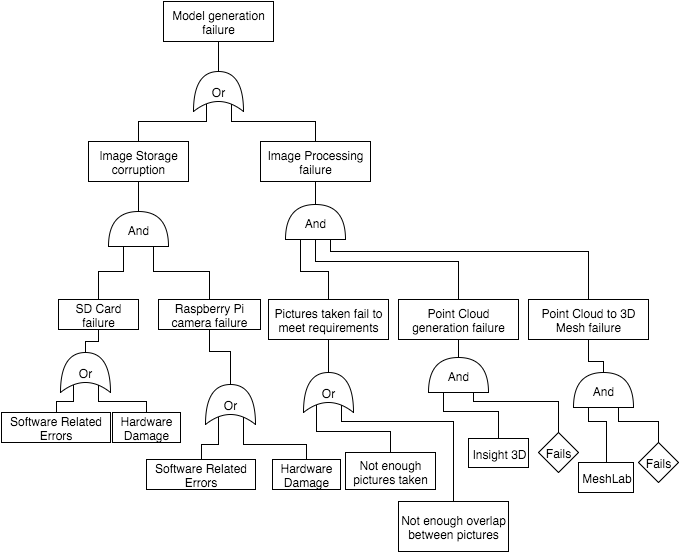
\includegraphics[width=\textwidth]{ModelFailure.png}}%
  \caption{Model Failure FTA}
  \label{fig:context_diagram}
\end{figure}

\newpage

\subsection{Unintended Flight Path}
 The figure below shows problems/situation where the quad-copter may travel in an unintended path.
\begin{figure}[h]
  \makebox[\textwidth][c]{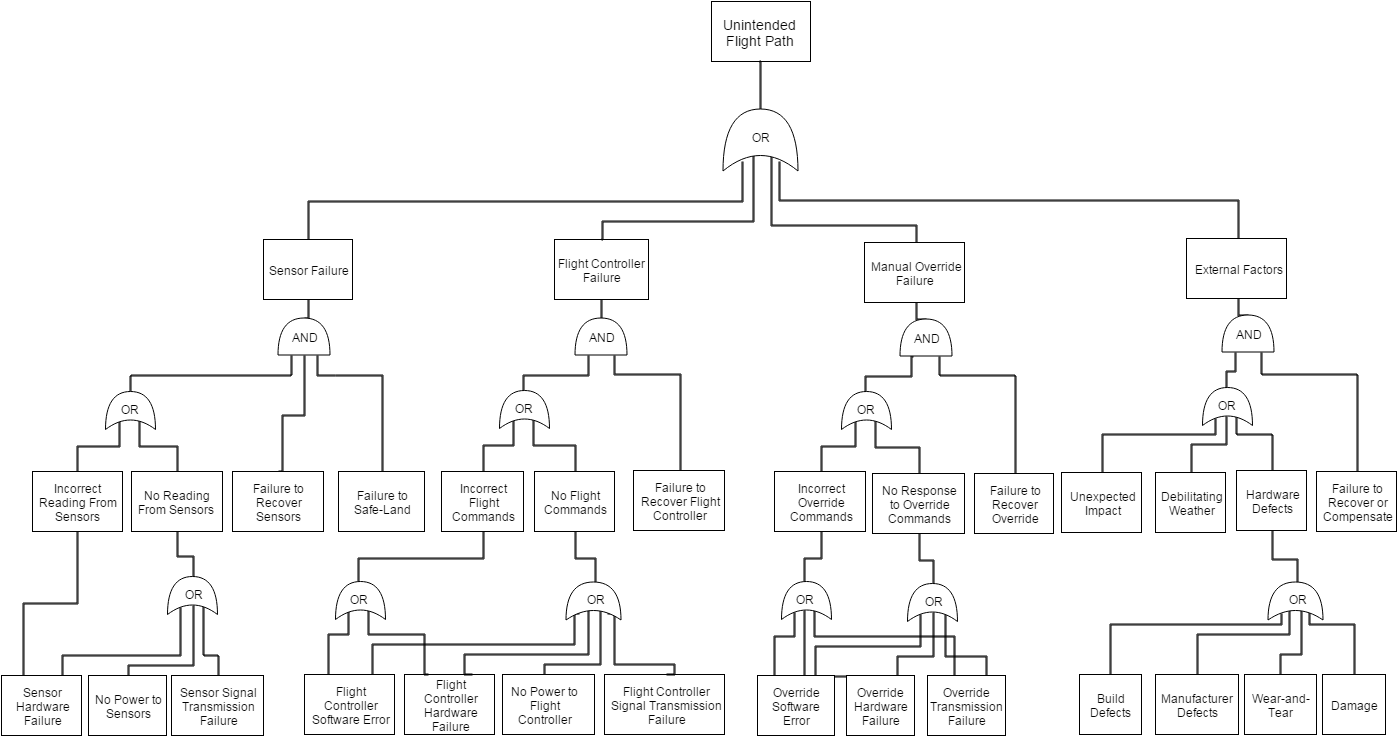
\includegraphics[width=0.95\paperwidth]{unintendedFlightPathNew.png}}
  \caption{Unintended Flight Path FTA}
  \label{fig:context_diagram}
\end{figure}
\newpage

\subsection{Unintended Landing}
The figure below shows problems/situations where the quad-copter may experience unintended landing.
\begin{figure}[h]
  \makebox[\textwidth][c]{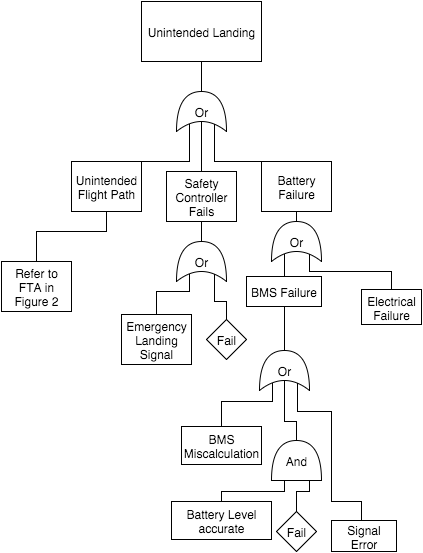
\includegraphics[width=0.6\textwidth]{Unintended_LandingFTA.png}}%
  \caption{Unintended Landing FTA}
  \label{fig:context_diagram}
\end{figure}

\newpage

\subsection{Injury to User}
The following figure shows the hazard analysis for situations that may lead to physical harm to the user.
\begin{figure}[h]
  \makebox[\textwidth][c]{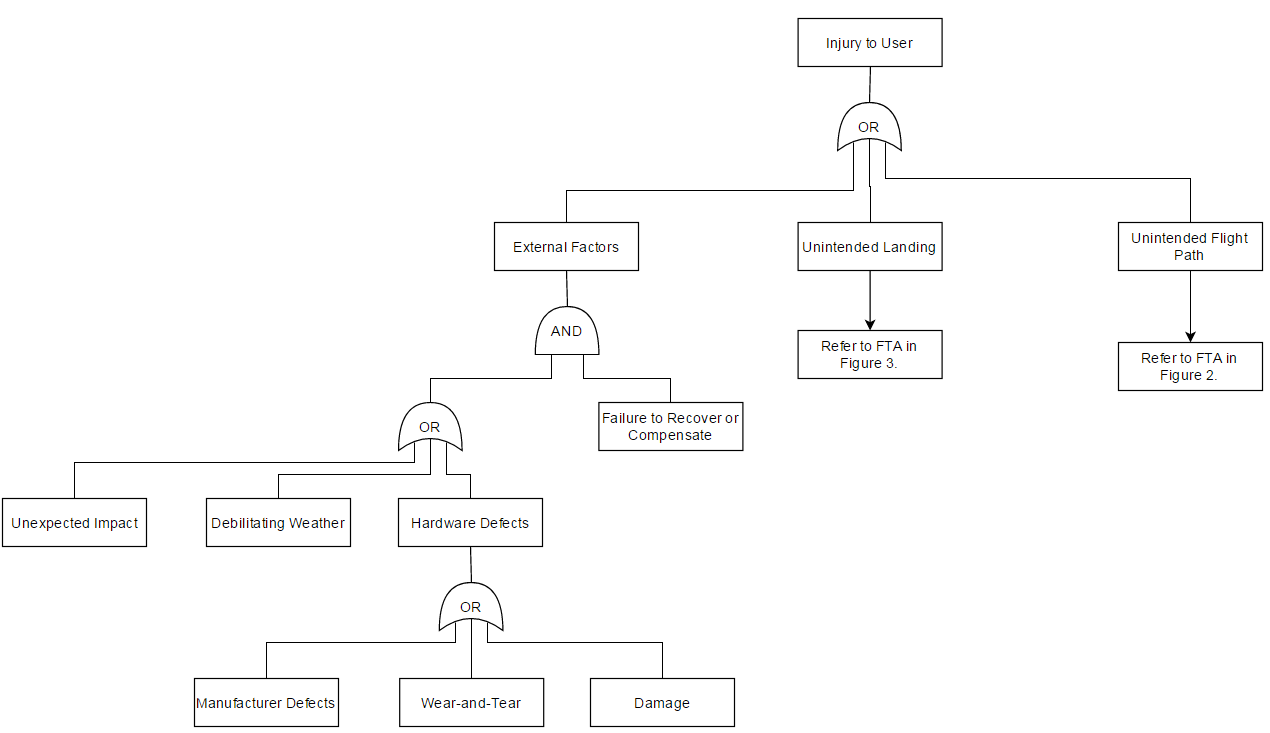
\includegraphics[width=1.65\textwidth]{InjurytoUserNew.PNG}}%
  \caption{Injury to user FTA}
  \label{fig:context_diagram}
\end{figure}
\newpage
\subsection{Unintended Take-off}
The following figure shows problems/situations where the quad-copter may experience unintended take-off.

\begin{figure}[h]
  \makebox[\textwidth][c]{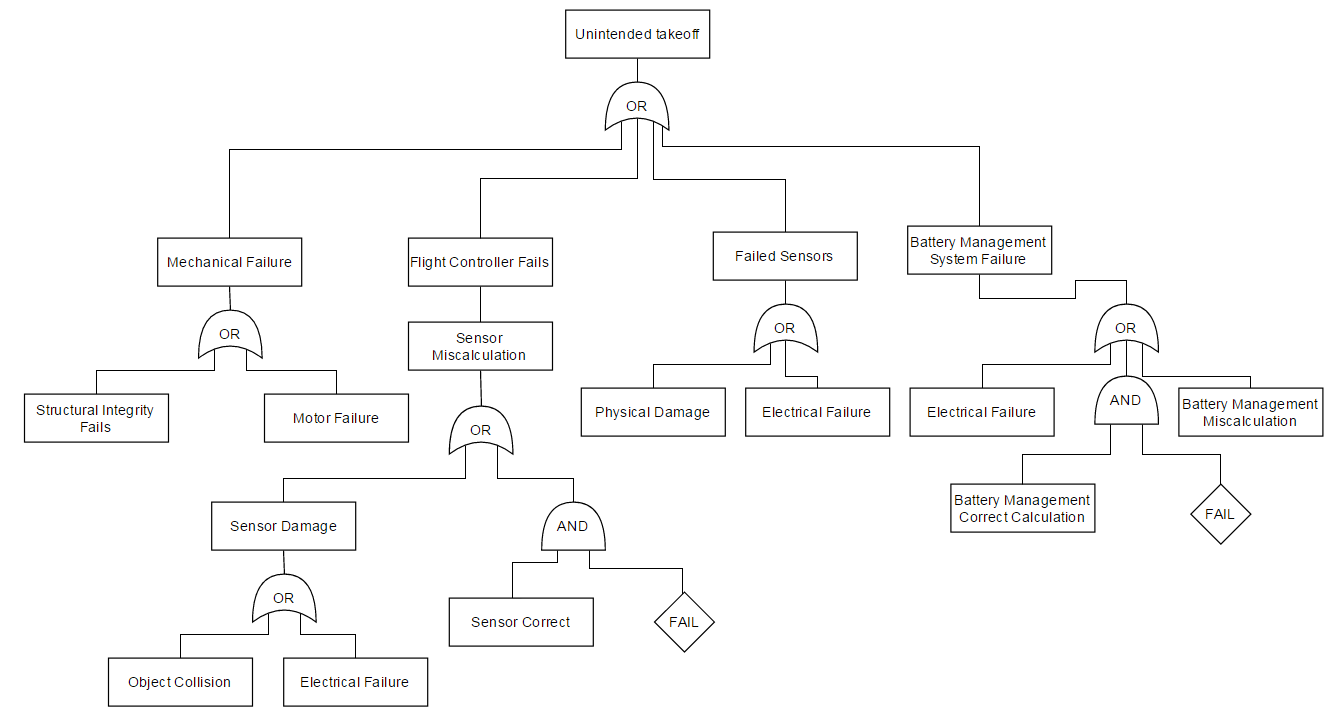
\includegraphics[width=1.65\textwidth]{UnintendedTakeOff.PNG}}%
  \caption{Unintended Take-off FTA}
  \label{fig:context_diagram}
\end{figure}

\newpage

\subsection{Take-Off Failure}
 The figure below shows problems/situation where the quad-copter may experience take-off failure.
\begin{figure}[h]
  \makebox[\textwidth][c]{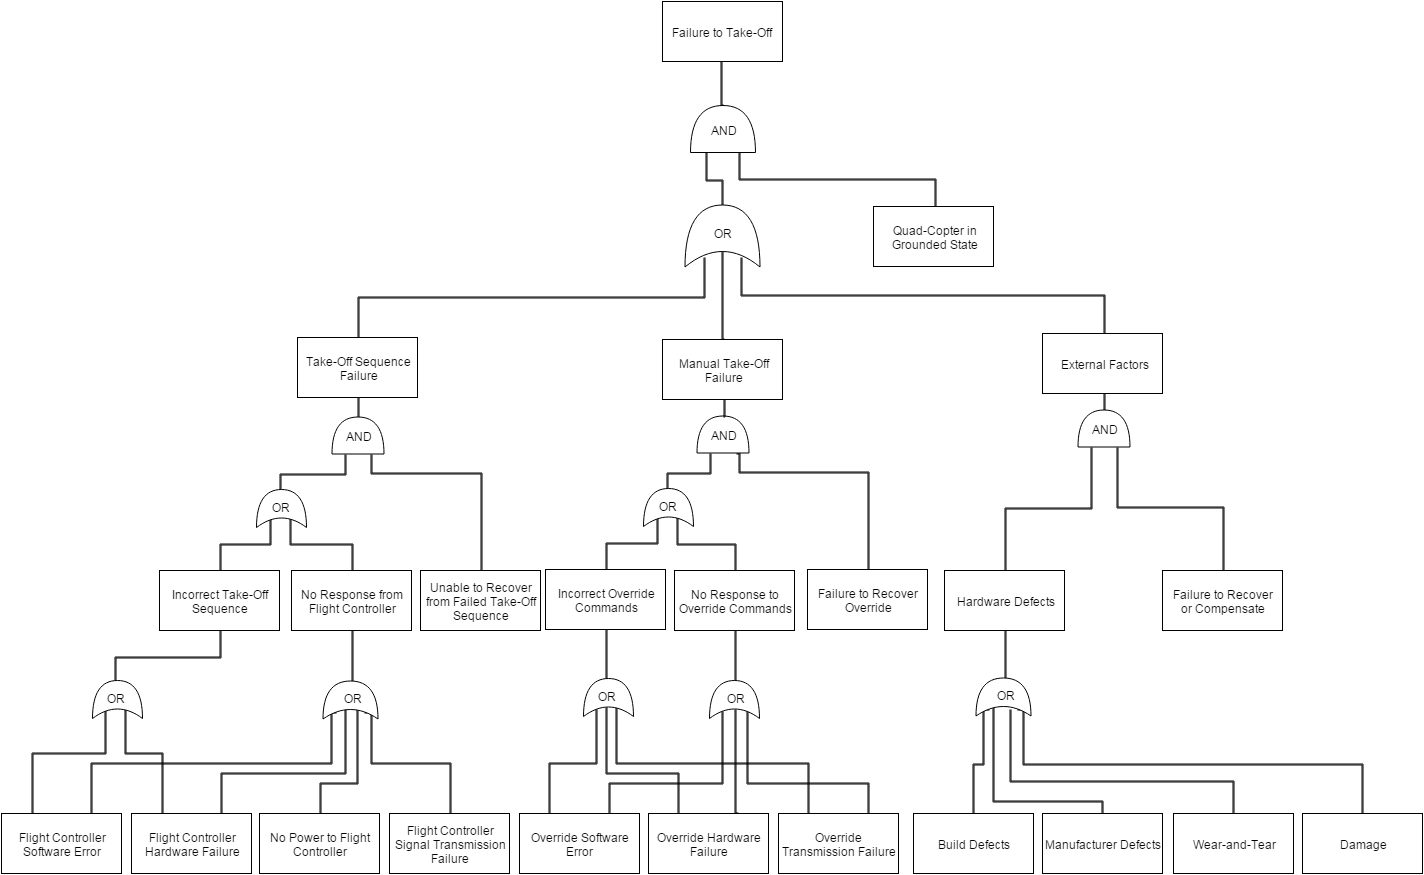
\includegraphics[width=0.95\paperwidth]{TakeOffFailure.png}}%
  \caption{Take-Off Failure FTA}
  \label{fig:context_diagram}
\end{figure}

\newpage


\subsection{General Hazard Handling}
\subsubsection{Object collision}
Handling object collision is complicated as the physical integrity of the components must be verified. Since the quad-copter will fly without a constant stream of user input, it is heavily reliant on the output of the sensors. In order to avoid catastrophic failure in regards to object collision, the state of the sensors must be continuously monitored. In the event damage occurs to the sensors, an emergency landing will be initiated to ensure that further damage does not occur.
\subsubsection{Electrical failure}
Electrical failure is a possibility due to the nature of the quad-copter. This could be caused by anything from a problem with the battery to there being problems with the physical electrical connections. In order to minimize the risk this poses we will have an initial check that is run prior to take off. In the event there is an issue with a component, the quad-copter will shut down.
\subsubsection{Sensor fails}
In the event the sensor gives erroneous output the user will have the option of initiating a manual override or allow the quad-copter to perform an emergency landing. These options ensures that if the orbit of the quad-copter does not seem correct or it is headed toward a possible collision, the user will be able to ensure that no additional damage to the quad-copter occurs.
\subsubsection{Emergency landing signal fails}
In the event the emergency landing signal ends up failing the user will have to initiate the manual override. This will require the user to pilot the quad-copter to a safe landing. Accidental triggering of the emergency landing signal would not cause any damage caused to the quad-copter, however diagnostics must be performed to determine the root of the erroneous signal and resolve it.
% \subsubsection{BMS miscalculation}
% A BMS (Battery Management System) miscalculation would be the result of an implementation error or hardware error. In the event it is an implementation error it would have to be solved through debugging the software component. The hardware error would be very difficult to deal with; because we would not be able to have a backup BMS attached to the quad-copter. We would have to ensure that through extensive testing that there are no problems with the BMS; in the event problems still arise with the BMS calculations, we would ensure the quad-copter stays grounded until the issues are resolved. This would involve monitoring the output of the BMS.
% \subsubsection{BMS readings are correct but there is a failure}
% In the event that the readings are accurate but the component fails we would have to ground the quad-copter until the problems with the component are resolved. This would involve monitoring the output of the BMS.
\subsubsection{Signal error}
In the event that a subsystem works perfectly; however, the signal it is outputting is incorrect we would have to debug the software component of the subsystem and ensure all physical connections pertaining to that subsystem. Again, to ensure no catastrophic damage occurs, the quad-copter must be grounded until the problems are resolved.
\subsubsection{Mechanical failure}
In the case of failure of the frame of the quad-copter, the connection between the frame and all components must be verified such that the none of the components are loose. The structural integrity of the frame itself must be verified to not have any cracks or deformations. In the case of a failure of the motors, a pre-flight check will be performed to ensure that all motors are functioning properly, otherwise the launch will be aborted.

\subsection{Model Generation Specific Hazard Handling}
\subsubsection{Software related errors}
The software related errors would have to resolved prior to the quad-copter taking flight. These errors would be resolved through extensive testing of the different components that will be interacting with the quad-copter. These problems would not put any person or the quad-copter in danger; furthermore, through trail runs we will be able to debug and resolve issues that may arise.

\subsubsection{Hardware damage}
Again certain components will need to be monitored to ensure that they are performing as intended. In the event these monitors detect abnormalities or lack of output, the user will be notified. If the component is a critical to the quad-copter (flight controller, sensors) then the quad-copter will initiate an emergency landing; otherwise upon completing the scan of an object the user will be notified of any problems that occurred.

\subsubsection{Poor picture quality}
The Raspberry Pi Camera will be set to take a picture at a fixed interval. In the event there are not enough pictures taken the interval can be set to a lower value. Inversely, if there are too many pictures being taken the interval can be increased. If the pictures that are taken are not of sufficient quality, i.e. they are blurred, poorly exposed, corrupted, etc., the camera settings may be modified before flight.

\newpage

\section{Failure Modes and Effects Analysis (FMEA)}
The failure modes and effects analysis is a bottom-up method of analyzing hazards in an attempt to determine the majority of methods in which a system may cause harm to its surroundings. The bellow sections focus on ways in which the EyeCopter may become hazardous during operation. 
\subsection{Function Overview}
The below figure illustrates the functional overview of the system followed by more detailed discussions regarding each leaf function.

\vspace{1cm}

\begin{figure}[h]
  \makebox[\textwidth][c]{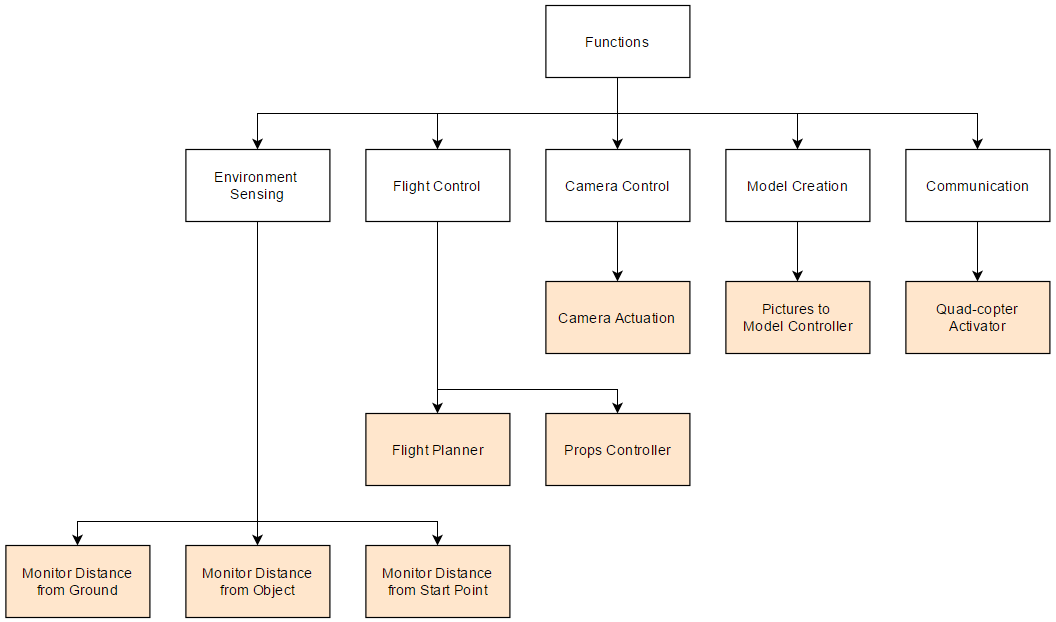
\includegraphics[width=1.5\textwidth]{FunctionalDecomposition.png}}%
  \caption{Functional overview diagram for EyeCopter system}
  \label{fig:context_diagram}
\end{figure}

\newpage

\subsubsection{Environment Sensing}
The functions under the subheading of "Environment Sensing" are used for the system to monitor the environment such that it can produce a correct flight plan to move around the object, and adjust its current flight path to fit to that flight plan accordingly.
\begin{table}[H]
  \begin{center}
   \makebox[\textwidth][c]{
      \begin{tabular}{p{6cm}p{8cm}}
          \multicolumn{1}{c}{\textbf{Function}} & \multicolumn{1}{c}{\textbf{Behaviour}} \\ \hline
          \textit{Monitor Distance from Ground} & 
          A function that monitors the readings from a downwards facing sensor on the quad-copter such that the quad-copter can be controlled and remains at a consistent height.\\ \hline 
          \textit{Monitor Distance from Object} & A function that monitors the distance from the object such that the flight path can be plotted around the object. \\ \hline 
          \textit{Monitor Distance from Start Point} & A function that estimates the position around the object such that the system knows when a revolution around the object is complete.
      \end{tabular}}
  \end{center}
  \caption[Environment sensing functional overview]{Environment sensing functional overview}
\end{table}

\subsubsection{Flight Control}
The Flight Control system consists of a CC3D flight control board as well as a micro-controller board used for flight planning.
\begin{table}[H]
  \begin{center}
   \makebox[\textwidth][c]{
      \begin{tabular}{p{6cm}p{8cm}}
          \multicolumn{1}{c}{\textbf{Function}} & \multicolumn{1}{c}{\textbf{Behaviour}} \\ \hline
          \textit{Flight Planner} & The flight planner is responsible for navigating the quad-copter around the object such that the camera is always facing the object and the quad-copter is at the correct distance away from the object. The flight planner uses proximity sensors on the front and sides to determine the distance from the object. The flight planner sends signals to the props controller corresponding to pitch, yaw, roll as well as throttle, much like a radio controller. \\ \hline 
          \textit{Props Controller} & The props controller is in charge of actuating the quad-copter's motors in such a way that the quad-copter will remain stable throughout the duration of the flight. The props controller uses an internal gyroscopic sensor to create a closed feedback loop in order to keep the quad-copter stable.
      \end{tabular}}
  \end{center}
  \caption[Flight control functional overview]{Flight control functional overview}
\end{table}

\subsubsection{Camera Control}
The camera as well as it's controllers may be found aboard the quad-copter.
\begin{table}[H]
  \begin{center}
   \makebox[\textwidth][c]{
      \begin{tabular}{p{6cm}p{8cm}}
          \multicolumn{1}{c}{\textbf{Function}} & \multicolumn{1}{c}{\textbf{Behaviour}} \\ \hline
          \textit{Camera Actuation} & The camera control determines whether or not the system is in the correct state and either begins taking pictures at regular intervals or ceases to take pictures all together. Pictures are saved progressively as they are taken to the available storage unit aboard the quad-copter and may be removed and accessed for model generating.
      \end{tabular}}
  \end{center}
  \caption[Camera control functional overview]{Camera control functional overview}
\end{table}

\subsubsection{Model Creation}
Model creation takes place on a separate computer included in the system but distinct from the quad-copter.
\begin{table}[H]
  \begin{center}
   \makebox[\textwidth][c]{
      \begin{tabular}{p{6cm}p{8cm}}
          \multicolumn{1}{c}{\textbf{Function}} & \multicolumn{1}{c}{\textbf{Behaviour}} \\ \hline
          \textit{Model Controller} & Model creation includes all processes necessary in order to generate a usable three dimensional model from the pictures taken by the quad-copter during flight. This encompasses importing the images, processing them as well as extracting a 3D model from the acquired data through the use of various tools (including \textit{insight3D} and \textit{Mesh Lab}).
      \end{tabular}}
  \end{center}
  \caption[Model creation functional overview]{Model creation functional overview}
\end{table}

\subsubsection{Communication}
Communications between the quad-copter and the manual controls are housed both on the quad-copter as well as within the remote control override.
\begin{table}[H]
  \begin{center}
   \makebox[\textwidth][c]{
      \begin{tabular}{p{6cm}p{8cm}}
          \multicolumn{1}{c}{\textbf{Function}} & \multicolumn{1}{c}{\textbf{Behaviour}} \\ \hline
          \textit{Quad-copter Activator} & The quad-copter activator's primary function is to alert the quad-copter that takeoff is to be achieved at a given time. This process includes turning on the quad-copter, initializing all components and ensuring that it is in the correct state.
      \end{tabular}}
  \end{center}
  \caption[Communication functional overview]{Communication functional overview}
\end{table}


\subsection{FMEA Charts}
The below failure modes and effects analysis charts depict possible hazards within the system in regards to each element of the  functional overview.
\subsubsection{Environment Sensing}
The following FMEA table considers the distance from the ground by interfacing with a downward sensor, and passes its data to the Flight Planner.
\begin{table}[H]
\footnotesize  
	\begin{adjustwidth}{-1.8in}{-1.8in}  
      \begin{center}
          \begin{tabular}{|p{3cm}p{3cm}p{3cm}p{3cm}p{4.5cm}|}
              \fmeaheader \\ \hline
              Sensor malfunction & 
              Unintended flight path & 
              \parbox[t]{3cm}{Hardware malfunction in sensor\\ Loose connection from sensor} &
              Monitor fluctuations in sensor readings  & 
              Enter SYSTEM\_LAND state. \\ \hline
              
              Ground out of sensor range & 
              Quad-copter will neither have data to maintain height, nor rise & 
              \parbox[t]{3cm}{Object to scan is too large.} &
              Monitor sensor readings for undefined readings.  & 
              Enter SYSTEM\_LAND state. \\ \hline
          \end{tabular}
      \end{center}
      \caption[Monitor Distance from Ground FMEA]{Monitor Distance from Ground FMEA}
    \end{adjustwidth}
\end{table}

The following FMEA table is specific to the function which monitors distance from the object. This function interfaces with a multiple forwards facing sensors, and passes its data to the Flight Planner.

\begin{table}[H]
\footnotesize  
	\begin{adjustwidth}{-1.8in}{-1.8in}  
      \begin{center}
          \begin{tabular}{|p{3cm}p{3cm}p{3cm}p{3cm}p{4.5cm}|}          
              \fmeaheader \\ \hline
              Sensor malfunction & 
              Unintended flight path & 
              \parbox[t]{3cm}{Hardware malfunction in sensor\\ Loose connection from sensor} &
              Monitor fluctuations in sensor readings and for sudden undefined or zero readings  & 
              Enter SYSTEM\_LAND state. \\ \hline 
              
              Sensor loses object & 
              Unintended flight path & 
              \parbox[t]{3cm}{Flight planner accelerates quad-copter too fast and the sensor no longer sees object \\ Flight planner turns too far and the sensor no longer sees object} &
              The reading from the sensor goes to the maximum value &
              Enter SYSTEM\_LAND state. \\ \hline 
          \end{tabular}
      \end{center}
      \caption[Monitor Distance from Object FMEA]{Monitor Distance from Object FMEA}
    \end{adjustwidth}
\end{table}

\newpage 

This function estimates the position of the quad-copter, such that the system will know when to rise and then begin executing another scan phase.
\begin{table}[H]
\footnotesize  
	\begin{adjustwidth}{-1.8in}{-1.8in}  
      \begin{center}
          \begin{tabular}{|p{3cm}p{3cm}p{3cm}p{3cm}p{4.5cm}|}
              \fmeaheader \\ \hline
              Incorrect calculation & 
              Scan phase never finishes & 
              Incorrect error calculations &
              Monitor length of scan phase and see if it goes abnormally long within the constraints of the system &
              Enter SYSTEM\_LAND state. \\ \hline 
              Incorrect calculation & 
              Scan phase completes early, not enough pictures taken & 
              Incorrect error calculations &
              Monitor length of scan phase and see if it is abnormally short&
              Continue SYSTEM\_SCAN state. \\ \hline 
          \end{tabular}
      \end{center}
      \caption[Monitor Distance from Start Point FMEA]{Monitor Distance from Start Point FMEA}
    \end{adjustwidth}
\end{table}

\subsubsection{Flight Control}
The flight planner controls the trajectory of the quad-copter around the object to be scanned. It does through an interface with the props controller.
\begin{table}[H]
\footnotesize  
	\begin{adjustwidth}{-1.8in}{-1.8in}  
      \begin{center}
          \begin{tabular}{|p{3cm}p{3cm}p{3cm}p{3cm}p{4.5cm}|}
              \fmeaheader \\ \hline
              Sensor malfunction & 
              Quad-copter flies away from object & 
              \parbox[t]{3cm}{Broken sensor \\ Poor connection \\ Misinterpreted data} & 
              Verify sensor is within expected bounds &
              Enter SYSTEM\_LAND state \\ \hline
              
              Communications malfunction & 
              Incorrect flight trajectory & 
              \parbox[t]{3cm}{Poor connection with flight planner \\ Corrupted data} & 
              Check if flight trajectory matches with planned trajectory within tolerance &
              Enter SYSTEM\_LAND state \\ \hline
          \end{tabular}
      \end{center}
      \caption[Flight Planner FMEA]{Flight Planner FMEA}
    \end{adjustwidth}
\end{table}

The props controller function ensures that the quad-copter is stable throughout the duration of the flight. It is responsible for moving the quad-copter in the direction specified by the flight planner.
\begin{table}[H]
\footnotesize  
	\begin{adjustwidth}{-1.8in}{-1.8in}  
      \begin{center}
          \begin{tabular}{|p{3cm}p{3cm}p{3cm}p{3cm}p{4.5cm}|}
              \fmeaheader \\ \hline
              
              Drive-train malfunction & 
              Unstable flight path &
              \parbox[t]{3cm}{Poorly fastened propeller or motor \\ Damaged propeller} &
              Check if flight trajectory matches with planned trajectory within tolerance &
              Enter SYSTEM\_LAND state
          	  \\ \hline
              
              Controls error & 
              Unstable flight path &
              \parbox[t]{3cm}{Outside force on quad-copter such as impact or turbulence} &
              Check if flight trajectory matches with planned trajectory within tolerance &
              Enter SYSTEM\_LAND state
          	  \\ \hline
          \end{tabular}
      \end{center}
      \caption[Props Controller FMEA]{Props Controller FMEA}
    \end{adjustwidth}
\end{table}

\newpage 

\subsubsection{Camera Control}
The below FMEA chart summarizes the hazards involved with the camera actuation. Notice that although an unpredictable or malfunctioning camera module may not present a direct hazard, the end result of an erroneous model may be hazardous depending on its intended application. Hence, all possible camera control failures are listed below in an attempt to ensure an accurate and non-hazardous final model.
\begin{table}[H]
\footnotesize  
	\begin{adjustwidth}{-1.8in}{-1.8in}  
      \begin{center}
          \begin{tabular}{|p{3cm}p{3cm}p{3cm}p{3cm}p{3cm}|}
          \fmeaheader \\ \hline
              Sensor malfunction & 
              Pictures taken of the object are too small & 
              \parbox[t]{3cm}{Broken sensor \\ Misinterpreted data \\ Adverse weather \\ Missed task} & 
              Erroneous sensor ``sanity check'' & 
              Exit picture taking state and attempt controlled landing with feedback alert. \\ \hline  
              
              Sensor malfunction & 
              Pictures taken of the object are too large (cannot see entire object) & 
              \parbox[t]{3cm}{Broken sensor \\ Misinterpreted data \\ Adverse weather \\ Missed task} & 
              Erroneous sensor ``sanity check'' & 
              Exit picture taking state and attempt controlled landing with feedback alert. \\ \hline  
              
              Camera malfunction & 
              Poor picture quality (blurred, poorly exposed...) & 
              \parbox[t]{3cm}{Damaged camera \\ Damaged lens \\ Corrupted data} & 
              Low-resolution or small image file sizes & 
              Exit picture taking state and attempt controlled landing with feedback alert. \\ \hline  
              
              Camera malfunction & 
              No pictures taken & 
              \parbox[t]{3cm}{Damaged camera \\ Damaged lens \\ Corrupted data} & 
              No saved image files & 
              Exit picture taking state and attempt controlled landing with feedback alert. \\ \hline  
              
              Incorrect state transition & 
              Pictures are taken before necessary (security hazard) & 
              \parbox[t]{3cm}{Damaged processor \\ Corrupted data} &
              Auditory shutter sound is active before expected & 
              Exit picture taking state and attempt controlled landing with feedback alert. \\ \hline  
              
              Incorrect state transition & 
              No pictures taken & 
              \parbox[t]{3cm}{Damaged camera \\ Damaged lens \\ Corrupted data \\ Damaged processor} & 
              No shutter sound is observed during flight & 
              Exit picture taking state and attempt controlled landing with feedback alert. \\ \hline  
              
              Timer malfunction & 
              Picture interval too short (overload on-board memory) & 
              \parbox[t]{3cm}{Damaged camera \\ Corrupted data \\ Damaged processor} & 
              Memory space fills too rapidly, sends alert & 
              Exit picture taking state and attempt controlled landing with feedback alert. \\ \hline  
              
              Timer malfunction & 
              Picture interval too long (large gap between pictures taken) & 
              \parbox[t]{3cm}{Damaged camera \\ Corrupted data \\ Damaged processor} &
              Memory space fills too slowly, sends alert & 
              Exit picture taking state and attempt controlled landing with feedback alert. \\ \hline  
              
              
          \end{tabular}
      \end{center}
      \caption[Camera Actuation FMEA]{Camera Actuation FMEA}
    \end{adjustwidth}
\end{table}

\newpage 

\subsubsection{Model Creation}
The below FMEA chart summarizes the hazards involved with the model controller. Notice that although an unpredictable or malfunctioning model controller may not present a direct hazard causing harm, the end result of an erroneous model may be hazardous depending on its intended application. Hence, all possible model control failures are listed below in an attempt to ensure an accurate and non-hazardous final model. 
\begin{table}[H]
\footnotesize  
	\begin{adjustwidth}{-1.8in}{-1.8in}  
      \begin{center}
          \begin{tabular}{|p{3cm}p{3cm}p{3cm}p{3cm}p{3cm}|}
              \fmeaheader \\ \hline
              
              Program Malfunction & 
              Incomplete model & 
              \parbox[t]{3cm}{Unusable pictures \\ Program Crashes \\ Insufficient resources} & 
              Program error warnings & 
              Exit model creation and return feedback alerts. \\ \hline  
              
              Program Malfunction & 
              Inaccurate model & 
              \parbox[t]{3cm}{Unusable pictures \\ Program Crashes \\ Insufficient resources} & 
              Program error warnings & 
              Exit model creation and return feedback alerts. \\ \hline  
              
              Program Malfunction & 
              Unbounded execution time & 
              \parbox[t]{3cm}{Unusable pictures \\ Program Crashes \\ Insufficient resources} & 
              Program error warnings & 
              Exit model creation and return feedback alerts. \\ \hline  
              
          \end{tabular}
      \end{center}
      \caption[Model Controller FMEA]{Model Controller FMEA}
    \end{adjustwidth}
\end{table}

\newpage 

\subsubsection{Communication}
The below FMEA chart summarizes the hazards involved with the quad-copter activator. Notice that although an unpredictable or malfunctioning quad-copter activator may not present a direct hazard causing harm, the end result of an erroneous model may be hazardous depending on its intended application. Hence, all possible quad-copter activator failures are listed below in an attempt to ensure an accurate and non-hazardous final model. 
\begin{table}[H]
\footnotesize  
	\begin{adjustwidth}{-1.8in}{-1.8in}  
      \begin{center}
          \begin{tabular}{|p{3cm}p{3cm}p{3cm}p{3cm}p{3cm}|}
             \fmeaheader \\ \hline
              
              Receiver Malfunction & 
              Incorrect signal received & 
              \parbox[t]{3cm}{Damaged receiver \\ Damaged transmitter \\ Corrupted data} &  
              Unexpected signal for current state & 
              Cut off communications, attempt to land quad-copter and return feedback alerts. \\ \hline  
              
              Receiver Malfunction & 
              Unintelligible signal received & 
              \parbox[t]{3cm}{Damaged receiver \\ Damaged transmitter \\ Corrupted data} &  
              Unexpected signal for current state & 
              Cut off communications, attempt to land quad-copter and return feedback alerts. \\ \hline  
              
              Receiver Malfunction & 
              No signal received & 
              \parbox[t]{3cm}{Damaged receiver \\ Damaged transmitter \\ Corrupted data} &  
              Unexpected signal for current state & 
              Cut off communications, attempt to land quad-copter and return feedback alerts. \\ \hline  
              
              Transmitter Malfunction & 
              Incorrect signal sent & 
              \parbox[t]{3cm}{Damaged receiver \\ Damaged transmitter \\ Corrupted data} &  
              Unexpected signal for current state & 
              Cut off communications, attempt to land quad-copter and return feedback alerts. \\ \hline  
              
              Transmitter Malfunction & 
              Unintelligible signal received & 
              \parbox[t]{3cm}{Damaged receiver \\ Damaged transmitter \\ Corrupted data} &  
              Unexpected signal for current state & 
              Cut off communications, attempt to land quad-copter and return feedback alerts. \\ \hline  
              
              Transmitter Malfunction & 
              No signal sent & 
              \parbox[t]{3cm}{Damaged receiver \\ Damaged transmitter \\ Corrupted data} &  
              Unexpected signal for current state & 
              Cut off communications, attempt to land quad-copter and return feedback alerts. \\ \hline  
              
              Radio Interference & 
              Loss of signal & 
              \parbox[t]{3cm}{Damaged receiver \\ Damaged transmitter \\ Corrupted data} &  
              Unexpected signal for current state & 
              Cut off communications, attempt to land quad-copter and return feedback alerts. \\ \hline  
              
              Radio Interference & 
              Signal corruption & 
              \parbox[t]{3cm}{Damaged receiver \\ Damaged transmitter \\ Corrupted data} &  
              Unexpected signal for current state & 
              Cut off communications, attempt to land quad-copter and return feedback alerts. \\ \hline  
              
          \end{tabular}
      \end{center}
      \caption[Quad-copter Activator FMEA]{Quad-copter Activator FMEA}
    \end{adjustwidth}
\end{table}



\newpage


\section{Further Safety Considerations}
Although many hazards have been addressed in the above sections, below are some that should be considered within (as well as outside) the context of the system.

\subsection{Spinning Propellers}
Quad-copters have an inherent danger of propellers spinning at high speeds. Under normal operating conditions, the quad-copter is not at risk of colliding with objects. However, at takeoff, landing, or any other time human operators are likely to be close to the quad-copter, there is as risk of harm associated with the props. This can be mitigated with a guard around the propellers to prevent unintentionally touching the blades at any time.
\subsection{Security}
Also to be noted is the ongoing issue of security violations involved when taking pictures in public. Ways of mitigating this however are difficult to identify as they are at the discretion of the user and are conditional upon the time, place and surroundings of the object being scanned as well as the object itself.






\end{document}